\section{Methodology}\label{sec:methodology}

\subsection{Overview}

This study uses an unsupervised deep clustering procedure that is based on multichannel spectrograms in order to extract features from particle trajectories and to automatically group particles. The workflow includes spectrogram construction, convolutional autoencoder pretraining, cluster-count selection and initialization, and deep clustering refinement with a reconstruction constraint.

This method is based on earlier work that involved the use of spectrograms and convolutional autoencoders for particle time-series analysis and adapts the input to six channels containing position, momentum, and electromagnetic field information~\cite{moreiraReport}. First, the standardized time series described in Section~\ref{sec:data} are converted into multichannel spectrograms. A reconstruction task then learns low-dimensional features, and then the number of clusters and initial cluster centers are determined. Finally, the representation and the assignment of particles are then improved by jointly optimizing the reconstruction and clustering losses.

The overall workflow is shown in Figure~\ref{fig:workflow}.

\subsection{Multichannel Spectrogram Construction}

A spectrogram is computed separately for each of the six standardized time series associated with each particle. The implementation uses the SciPy spectrogram function with a window length of 256 samples and a hop size of 128 samples, corresponding to 50\% overlap between adjacent windows. A Tukey window with a shape parameter of 0.25 is used, and the mean is removed within each window. A one-sided magnitude spectrum is returned. The sampling frequency is set to one, so frequencies are expressed in cycles per sampled point~\cite{scipySpectrogram}.

The magnitude spectrum is transformed according to

\begin{equation} S_{\log}=\log(1+S), \end{equation}

where \(S\) denotes the magnitude spectrum. This transformation compresses its numerical dynamic range before network processing.

For a time series with 2,004 samples, these settings produce 129 frequency bins and 14 time windows. Only complete windows are used, without padding at the end of the sequence; the leftover samples do not constitute an extra frame. Bilinear interpolation subsequently resizes the log-magnitude spectrogram to a fixed \(33\times60\) grid. This resampling process acts on the existing representation and does not add any new independent temporal or spectral information.

The resized spectrograms are standardized separately for each channel by the mean and standard deviation computed across all particles and all spectrogram grid points in that channel. The six channels are then combined into an input tensor of size \(6\times33\times60\) for each particle. Figure~\ref{fig:spectrogram} illustrates the resulting six-channel input for one particle.

\begin{figure}[htbp]
\centering
\figureasset[\linewidth]{figures/input-log-spectrogram-example.png}{Six-channel spectrogram input for an example particle}
\caption[Six-channel spectrogram input for an example particle]{Six-channel spectrogram input for an example particle. The panels correspond to \(x\), \(p_x\), \(p_y\), \(E_x\), \(E_y\), and \(B_z\). Each time series is transformed into a magnitude spectrogram, logarithmically compressed, resized, and standardized channel-wise to form the convolutional autoencoder input. The horizontal and vertical axes indicate the resized time-bin and frequency-bin indices, respectively. Colors represent standardized log-magnitude values, with an independent color scale for each panel.}\label{fig:spectrogram}
\end{figure}

\subsection{Convolutional Autoencoder and Reconstruction Pretraining}

The convolutional autoencoder has an encoder and a decoder. The encoder compresses the multichannel spectrogram into a low-dimensional feature vector, and the decoder reconstructs the input from that vector. The feature representation used for the subsequent clustering is obtained by minimizing the reconstruction error.

For particle \(i\), let \(X_i\) denote its six-channel spectrogram input. With encoder \(f_\theta\) and decoder \(g_\phi\), the latent representation and reconstruction are

\begin{equation} z_i=f_\theta(X_i), \qquad \widehat{X}_i=g_\phi(z_i), \end{equation}

where \(z_i\in\mathbb{R}^{32}\), and \(\theta\) and \(\phi\) are the trainable encoder and decoder parameters, respectively.

The encoder contains four two-dimensional convolutional layers with 8, 16, 32, and 64 output channels. Each layer uses a \(3\times3\) kernel, a stride of two, padding of one, and a ReLU activation. The final convolutional output is flattened and mapped to a 32-dimensional feature vector through a linear fully connected layer.

The decoder first maps the latent vector back to the convolutional feature dimensions through a fully connected layer. Four transposed convolutional layers then reconstruct the multichannel representation. ReLU activations follow the first three transposed convolutional layers, while the final layer has no non-negative activation constraint, and thus is able to reconstruct standardized inputs that include negative values. Bilinear interpolation adjusts the output to the original input dimensions. A summary of the main architecture can be found in Table~\ref{tab:architecture} in Appendix~\ref{app:implementation}.

Pretraining minimizes a channel-weighted mean squared error:

\begin{equation} L_{\mathrm{recon}} = \frac{ \displaystyle \sum_{i\in\mathcal{B}} \sum_{c=1}^{C} w_c \left\|\widehat{X}_{i,c}-X_{i,c}\right\|_F^2 }{ BHW\displaystyle\sum_{c=1}^{C}w_c }, \end{equation}

where \(\mathcal{B}\) denotes the current batch, \(B\) is its number of samples, \(C=6\) is the number of channels, and \(H=33\) and \(W=60\) are the spectrogram grid dimensions. The squared Frobenius norm sums the squared reconstruction errors over all grid points within a channel.

For the channel ordering \(x,p_x,p_y,E_x,E_y,B_z\), the weights are

\begin{equation} \boldsymbol{w}=(1,\;1,\;1,\;0.2,\;0.2,\;1). \end{equation}

This configuration reduces the relative contribution of electric-field reconstruction errors to the training objective while retaining all six channels as inputs.

During pretraining, particles are randomly divided into an 80\% training subset and a 20\% validation subset, which contain 10,240 and 2,560 particles, respectively. Training uses the Adam optimizer with a learning rate of \(10^{-3}\), a batch size of 64, and a maximum of 200 epochs. Pretraining stops when the validation loss has not improved for 15 consecutive epochs. The model with the lowest validation loss is selected for subsequent clustering.

This split is used to monitor reconstruction training. The fact that the standardization parameters are calculated from the whole analysis dataset means that the validation subset is not regarded as an independent generalization test set.

\subsection{Cluster-Count Selection and Initialization}

After pretraining, the encoder extracts 32-dimensional features for all particles. \(K\)-means is then used in this feature space for each possible number of clusters \(K\) ranging from 2 to 12. For each candidate configuration, there are 100 initializations, and each initialization is carried out for a maximum of 1,000 iterations. The solution that has the smallest within-cluster sum of squared distances is kept.

For a candidate cluster count \(K\), the \(K\)-means inertia is

\begin{equation} I(K) = \sum_{i=1}^{N} \left\|z_i-\mu_{a_i}\right\|_2^2, \end{equation}

where \(N\) is the number of particles, \(a_i\) is the \(K\)-means assignment of particle \(i\), and \(\mu_{a_i}\) is the corresponding cluster center.

The elbow criterion, which is based on log inertia, is used to determine the number of clusters. The proposed numbers of clusters and their corresponding log-inertia values are each rescaled independently to the range \([0,1]\). Then the perpendicular distance from each of the resulting points to the line joining the first and last of the candidate points is calculated, and the candidate having the greatest distance is chosen as the elbow.

Silhouettes are also calculated for the candidate configurations as additional information; the maximum of these values is not employed in determining \(K\). After the number of clusters has been chosen, the respective \(K\)-means centers are used to initialize the deep clustering layer.

Figure~\ref{fig:cluster-count-selection} shows the corresponding diagnostics for the pretrained spectrogram representation. The elbow criterion selects \(K=5\), which does not maximize the sampled silhouette score over the candidate range. These silhouette values describe \(K\)-means assignments before DEC refinement and are distinct from the final clustering scores reported in Section~\ref{sec:silhouette-results}.

\begin{figure}[htbp]
\centering
\begin{subfigure}[t]{0.49\linewidth}
\centering
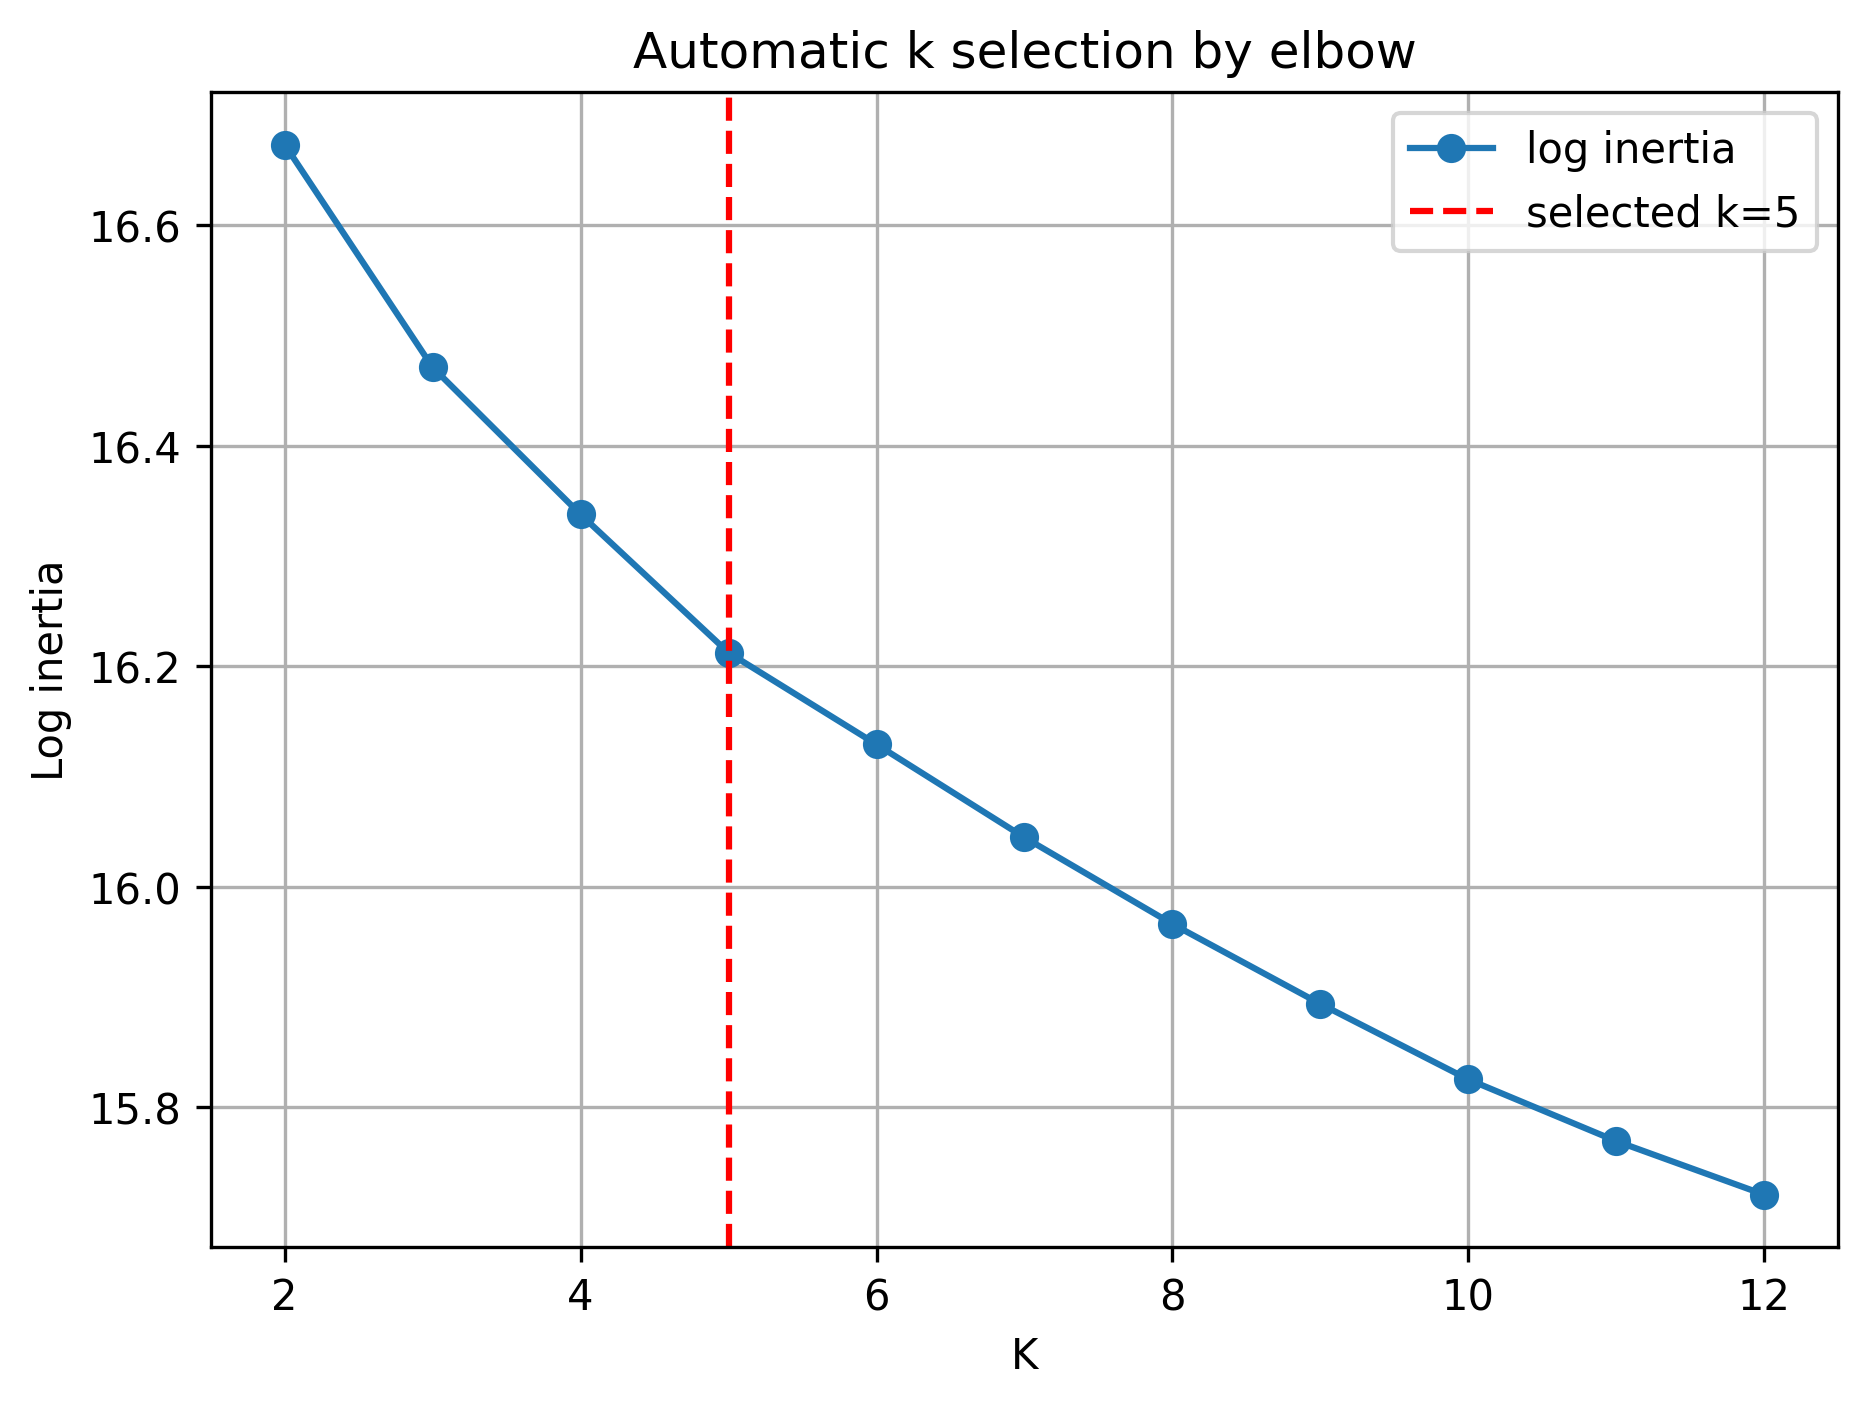
\includegraphics[width=\linewidth]{figures/cluster-count-elbow.png}
\caption{Log inertia and elbow-selected cluster count.}
\end{subfigure}\hfill
\begin{subfigure}[t]{0.49\linewidth}
\centering
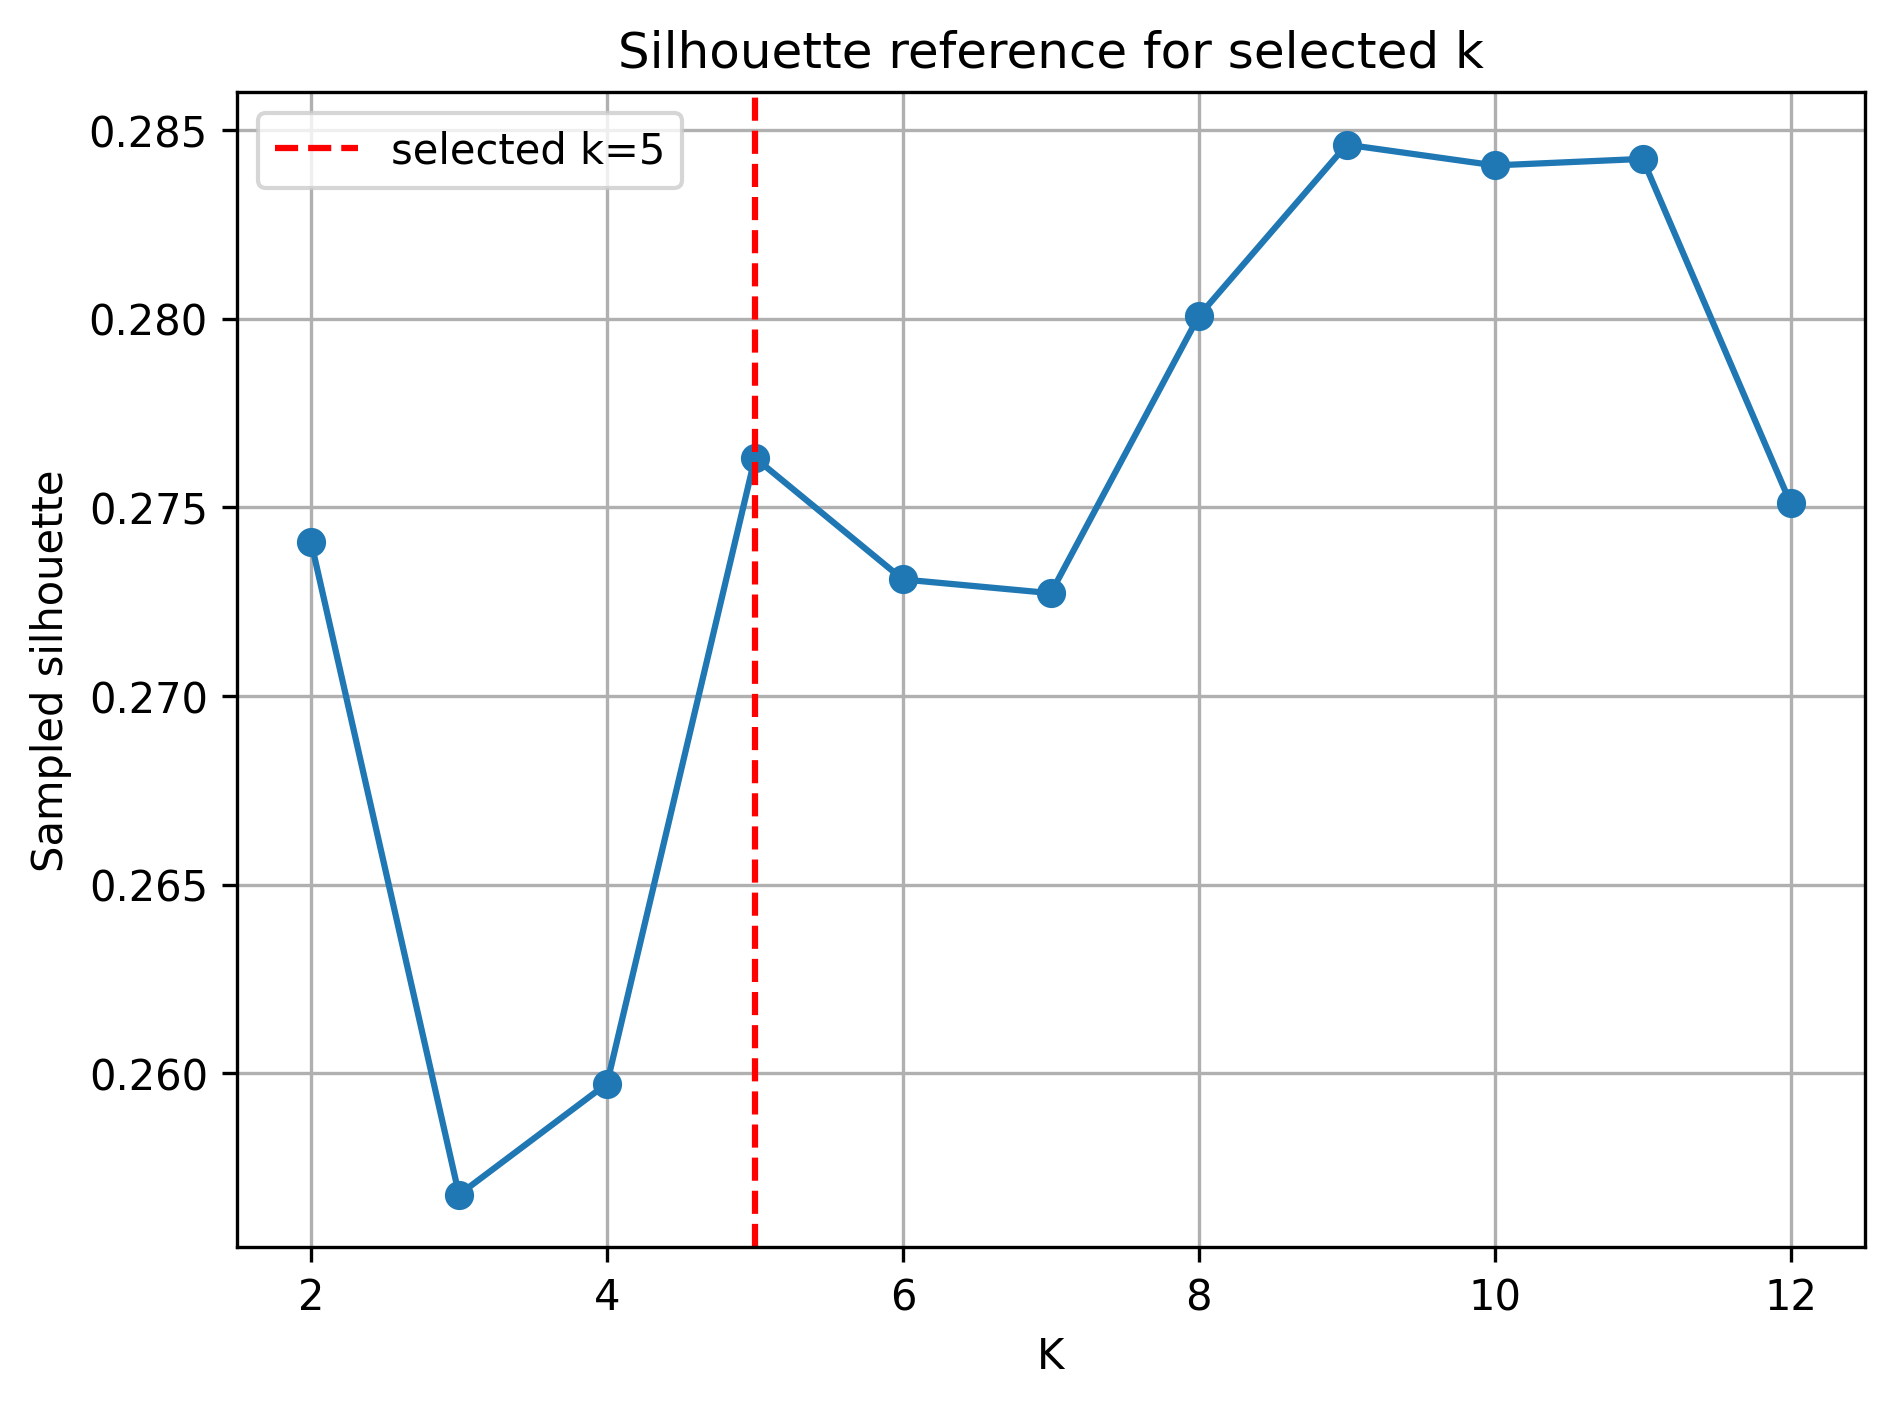
\includegraphics[width=\linewidth]{figures/cluster-count-silhouette.png}
\caption{Sampled silhouette scores for reference.}
\end{subfigure}
\caption[Cluster-count selection in the pretrained spectrogram latent space]{Cluster-count diagnostics for K-means in the 32-dimensional pretrained spectrogram latent space, before DEC refinement. (a) Log inertia for candidate counts \(K=2,\ldots,12\); the normalized elbow criterion selects \(K=5\). (b) Sampled silhouette scores for the same candidate counts, shown only as supplementary information rather than as the selection criterion. The red dashed line marks the elbow-selected count in both panels.}
\label{fig:cluster-count-selection}
\end{figure}

\subsection{Deep Clustering Refinement with a Reconstruction Constraint}

Clustering refinement follows the soft-assignment and target-distribution update procedure of DEC. Given particle features \(z_i\) and cluster centers \(\mu_j\), soft assignments are calculated using Student's t-distribution:

\begin{equation} q_{ij} = \frac{ \left(1+\|z_i-\mu_j\|_2^2/\alpha\right)^{-(\alpha+1)/2} }{ \displaystyle\sum_{k=1}^{K} \left(1+\|z_i-\mu_k\|_2^2/\alpha\right)^{-(\alpha+1)/2} }, \qquad \alpha=1. \end{equation}

Here, \(q_{ij}\) represents the soft assignment of particle \(i\) to cluster \(j\), with assignments summing to one for each particle~\cite{xie2016}.

An auxiliary target distribution is constructed from the current assignments:

\begin{equation} f_j=\sum_{i=1}^{N}q_{ij}, \qquad p_{ij} = \frac{q_{ij}^{\,2}/f_j} {\displaystyle\sum_{k=1}^{K}q_{ik}^{\,2}/f_k}. \end{equation}

The quantity \(f_j\) is the total soft-assignment mass of cluster \(j\). Squaring the assignments emphasizes higher-confidence memberships, while normalization by cluster frequency adjusts the relative contributions of different clusters. The target distribution is calculated using all particles and updated after each epoch; it stays constant during the next epoch's gradient updates and is not included in backpropagation.

The decoder and reconstruction loss are retained during clustering refinement to constrain changes to the input representation. Combining reconstruction and clustering objectives follows the structure preservation approach introduced in IDEC~\cite{guo2017}.

The clustering loss for the current batch is

\begin{equation} L_{\mathrm{cluster}} = \sum_{i\in\mathcal{B}} \sum_{j=1}^{K} p_{ij}\log\frac{p_{ij}}{q_{ij}}. \end{equation}

The joint training objective is

\begin{equation} L = L_{\mathrm{recon}} + \lambda L_{\mathrm{cluster}}, \qquad \lambda=5\times10^{-4}. \end{equation}

The reconstruction term is the channel-weighted loss used during pretraining. The KL term is summed up over the particles and clusters in the present batch and not averaged over the particles, so its coefficient has to be understood in conjunction with the loss reduction and the batch size, which is fixed at 64.

This report uses the reconstruction-plus-weighted-clustering form used in the previous one. The coefficient chosen in this case resulted from exploratory comparisons of the clustering weights. Because of differences in input standardization, the weighting of the reconstruction, and the KL reduction, there is no direct numerical agreement with the coefficient given in the earlier study.

During refinement, a randomly chosen half of the particles---that is, 6,400 samples---participate in the gradient updates. For all 12,800 particles, the soft assignments and the target distributions are calculated both at the beginning of training and after each epoch. As a result, particles left out of the refinement gradient updates still help construct the target distributions and are not treated as an independent test set.

Refinement uses Adam with a learning rate of \(10^{-3}\). The reconstruction loss updates the encoder and decoder, while the clustering loss updates the encoder and cluster centers. Final labels are obtained from the soft assignments:

\begin{equation} y_i=\underset{j}{\arg\max}\;q_{ij}. \end{equation}

These discrete labels are used for output and monitoring and do not participate in gradient computation. Figure~\ref{fig:architecture} illustrates the model structure and these dependencies.

\begin{figure}[htbp]
\centering
\figureasset[\linewidth]{figures/architecture.png}{Convolutional autoencoder and reconstruction-constrained deep clustering}
\caption[Convolutional autoencoder and reconstruction-constrained deep clustering]{Convolutional autoencoder and deep clustering refinement with a reconstruction constraint. The encoder maps each six-channel spectrogram to a 32-dimensional representation, from which the decoder reconstructs the input. Latent features and cluster centers jointly determine soft assignments \(Q\), which are used to construct the auxiliary target distribution \(P\). Training combines a channel-weighted reconstruction loss with a KL clustering loss using \(\lambda=5\times10^{-4}\). The KL term is summed over minibatch particles and clusters. Reconstruction updates the encoder and decoder, while clustering updates the encoder and cluster centers. Final labels are obtained by selecting the largest soft assignment for each particle. Spectrograms, latent features, and cluster distributions in the diagram are schematic.}\label{fig:architecture}
\end{figure}

\subsection{Training Monitoring and Model Selection}

The final configuration performs 350 epochs of deep clustering refinement. Total loss, reconstruction loss, the unweighted KL term, and its weighted contribution are recorded at each epoch. Changes in particle assignments are also monitored.

The label-change rate between consecutive epochs is defined as

\begin{equation} \delta^{(t)} = \frac{1}{N} \sum_{i=1}^{N} \mathbf{1} \left[ y_i^{(t)}\neq y_i^{(t-1)} \right], \end{equation}

where \(\mathbf{1}[\cdot]\) is the indicator function. This metric gives the fraction of particles reassigned between consecutive epochs. Refinement runs for the prescribed number of epochs; the label-change rate is used as a diagnostic and does not trigger early stopping.

Following each epoch, the silhouette score is calculated by means of Euclidean distances within the present latent space, based on a subset of 5,000 particles that are selected using a fixed random seed. This score serves both as a means of monitoring the training process and as a basis for model selection, with the candidate that has the highest score being kept. The score's interpretation with regard to within-cluster cohesion and between-cluster separation is in accordance with Rousseeuw's definition~\cite{rousseeuw1987}.

Once the model has been selected, final labels are assigned to all the particles, and the silhouette score is then recalculated on a subset consisting of 10,000 particles. It is for this reason that the final score reported might differ slightly from the score obtained during epoch-level monitoring. Since the model selection and the final evaluation both make use of the same analysis dataset, these scores are given as internal clustering assessments and not as independent test results.

The workflow keeps the representations and labels that were obtained before refinement, along with the losses at each epoch and the changes in assignment. The final outputs consist of the particle identifiers, the cluster labels, the latent features, the sampling settings, and the loss weights, which enable the assignments to be linked to the original trajectories. The key settings are given in Table~\ref{tab:settings} in Appendix~\ref{app:implementation}.
